% Chapter 3

\chapter{Dataset} % Write in your own chapter title
\label{Chapter3}
\lhead{Chapter 3. \emph{Dataset}} % Write in your own chapter title to set the page header

\section {Dataset Description}
To determine the indoor location of the user, we need a trained model on specific dataset  through which we can predict his location. In order to train our model, we gathered dataset which contains the fingerprints of BLE beacons in Computer Engineering Department. Each beacon has its own MAC address which is used for its identificati n. We have total 24 beacons, that’s why we have 24 input features and each feature contains the RSSI values of specific beacon associated with that feature, and the output is the labeled name of the location. We have total 23 labels which mean we have total 23 classes hence it is a multiclassification problem. RSSI values ranges from -95dBm (low RSSI ~ far off Access point) to - 50dBm (demonstrating high RSSI close to Access point).
\begin{figure}[h]
  		\centering
    		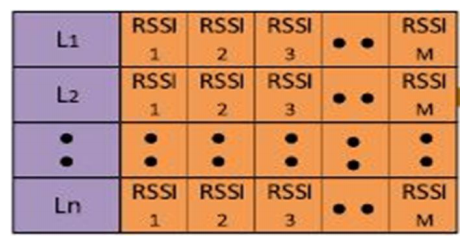
\includegraphics{./Figures/1}
\caption{Dataset format with each label and its corresponding RSSI value}
\label{fig:1}
 		\end{figure}
    

\section {Experimental Area Description}
The experimental area that we covered is the Computer Engineering building of UET, LHR. We skip some rooms of that building because they are locked most of the time. The representation of the deployment of beacons in dept is shown in the following figures. Figure 2 represents the ground floor and Figure 3 represents 1st floor of the building. Small blue circle represent BLE beacon. Following figures only represents those rooms that we have considered in our experimental area. Each room is assigned a label as shown in the figures. Corridors are divided into 4 portions. Each portion is represented by a dotted box and assigned a label shown in the figures. 
\begin{figure}[h]
  		\centering
    		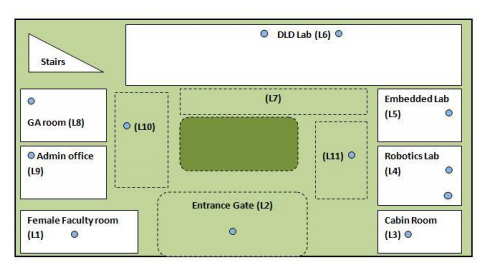
\includegraphics{./Figures/2}
\caption{Map of ground floor of the building where beacons are installed}
\label{fig:2}
 		\end{figure}
    \begin{figure}[h]
  		\centering
    		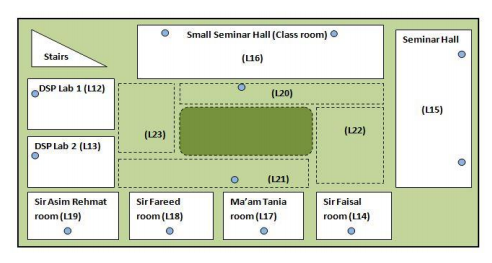
\includegraphics{./Figures/3}
\caption{Map of first floor of the building where beacons are installed}
\label{fig:3}
 		\end{figure}
 \section {Collected Dataset}
Our collected dataset contains 6500 samples of 18 locations of selected area out of 23 locations. Each  location has its own fingerprint RSSI value with respect to certain beacon which depends on different environmental conditions such as distance of device location from the beacon or signal capturing strength of the device. So, we collect samples to predict different locations. The number of samples collected per location is shown in the following figure.
 \begin{figure}[h]
  		\centering
    		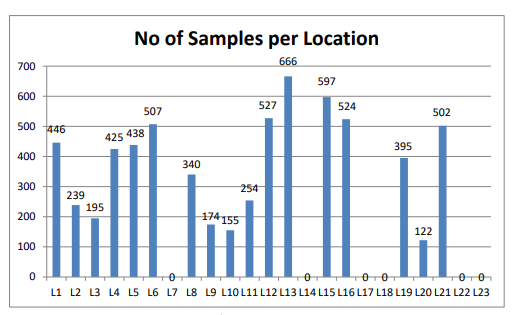
\includegraphics{./Figures/4}
\caption{Number of samples collected for each label}
\label{fig:4}
 		\end{figure}
\\\\
\subsection{Preparation of data set}
When we captured the data, numerous .csv files generated in which each .csv file contain one sample. We used 5 different cell phones for data capturing. Then we compile all the generated .csv files into single .csv file in specific format that we have shown in Figure 1. We discard all those RSSI values of surrounding BLE enable devices which are not from our BLE beacons.
\subsection{Preprocessing of data}
We have done pre-processing on our collected data set. In pre-processing, we have dropped all those rows that have null values in all of their input columns. During data collection some access points are visible, some not hence there were lot of missing values in data set. So, we replace missing values with -100dbm. The reason for replacing the missing values with -100dbm is because it shows extremely weak signal means it is far off from access point. We have not done normalization on our data set because we didn’t find it suitable for our collected dataset.


\subsection{Performance Measures criterion for the comparison of algorithms}
{\bf Accuracy} is the measurement of model performance. It is calculated as the no of samples correctly classified/ total no of samples.
 
\begin{figure}[h]
  		\centering
    		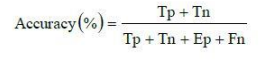
\includegraphics{./Figures/accuracy}
\caption{Accuracy}
\label{fig:5}
 		\end{figure}

{\bf Precision} tells about how accurate your model is out of those predicted positive, how many of them are true positive. Precision is a good measure to determine, when the costs of False Positive is high.

\begin{figure}[h]
  		\centering
    		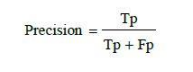
\includegraphics{./Figures/precision}
\caption{Precision}
\label{fig:6}
 		\end{figure}
 
{\bf Recall} actually calculates how many of the Actual Poitives our model captures through labeling it as Positive (True Positive).

\begin{figure}[h]
  		\centering
    		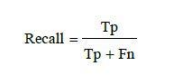
\includegraphics{./Figures/recall}
\caption{Recall}
\label{fig:7}
 		\end{figure}

For calculation of precision and recall for multi-classification, we can calculate the precision and recall separately for each class.
% For example, for class X, we can calculate its precision like that TP_X/Total Predicted X and recall for X class is calculated as TP_X/Total Actually Labeled X.
Then we calculate the average precision and recall of all classes and hence we will get the approximate calculation of precision and recall for them. 